\chapter{Proposta}\label{cap4}

\section{Usuários}

Pessoas e instituições estão se afastando cada vez mais de impressões e se aproximando de livros eletrônicos. Os e-books estão fazendo sucesso e estão cada vez mais sendo utilizado pelos editores para tornar disponíveis livros em formato eletrônico. Eles oferecem benefícios para os leitores incluindo a redução de danos ao meio ambiente, a portabilidade, o peso leve e ao reforço da capacidade de referência. Mas, para alguns leitores, e-books oferecem ainda mais: a sua primeira oportunidade de desfrutar da leitura. Essa pessoas com algum tipo de limitação, seja cego ou com baixa visão, pessoas com dislexia ou outras dificuldades de aprendizagem ou ainda que não conseguem segurar ou mudar a página de um livro encontram enormes dificuldades para ler livros impressos e, dependendo do caso, tal prática torna-se impossível \cite{chronicle}.

Neste contexto este mecanismo de semântica e ontologia proposto, poderia auxiliar os usuários de audiobooks a possuírem maior mobilidade e conforto ao dispor destas tecnologias.

\section{Terminologias Existentes}

\subsection{Ontologias Existente}
Ontologias para a organização de \textit{audiobooks} são raras. Porém há uma grande similaridade entre ontologias para livros e para \textit{audiobooks}, uma vez que que tanto o livro quanto o áudio descrevem o mesmo conteudo. Mundando unicamente a forma que disponibilizam esse material. Dessa forma, a ontologia usada - nesse trabalho - para organizar ontologicamente um audiobook foi baseada uma ontologia desenvolvida por Naveen Kumar no intituto \textit{Ambedkar Institute of Advanced Communication Technologies}. 

A ontologia desenvolvida em Ambedkar deve cobrir uma ampla quantidade de informações e deve ter a capacidade para especificar as informções de formar a tornar mais eficas a pesquisa\cite{ontologybook}. A figura 2 mostra a abstração basica dos conceitos relacionados à livros e as relações semânticas. 

Existem basicamente quatro relações entre os conceitos: a relação de herança, relação de instância, relação parte-todo e relação sinoníma. A Relação de herança revela a relação de inclusão entre conceitos, ou seja, um subi-conceito é uma espécie de conceito pai, como por exemplo: ``Ruby of Rails'' é uma espécie de ``livro técnico'', em que ``livro técnico'' é um conceito pai, e ``Ruby of Rails'' é a sub-classe. A relação de instância é a relação da existência especifica de um conceito, como ``livro departamento de TI'' é uma instância de ``livro computador''. Relação parte-todo expressa um conceito que faz parte de um outro conceito, como ``manual de laboratório'' é parte do ``livro departamento de eletrônica''.

Não há informação semântica rica descrito explicitamente na ontologia. Podemos conhecer a partir da Figura 2 que o Java é um livro departamento CSE de livros de informática, e as pessoas podem chamá-lo pelo nome de ``OAK''. RDF (Resource Description Framework) e RDFS (RDF Schema) é um modelo de dados e mecanismo de apoio para a representação de meta-dados de esquemas \cite{rdf}, e é uma linguagem de representação de ontologias. RDF é um padrão baseado em XML para descrever recursos que existem na web, intranets e extranets. RDFS é usado para criar vocabulários que descrevem grupos de recursos RDF relacionados e as relações entre esses recursos. 


 \begin{figure}[ht]
	\centering
		\includegraphics[keepaspectratio=true,scale=0.5]{figuras/ontology.eps}
	\caption{Uma pequena parte da ontologia no dominio de livros.}
	\label{lanctocalivros}
\end{figure}

\section{Descrição do Ambiente Web}
Audiobook, basicamente são livros narrados. Ou seja, são gravações dos conteúdos de livros, cujo o mesmo é lido. Estes audiobook posuem diversos formatos informacionais, como MP3 e WMA, entre outro, podendo ser pagos ou gratuitos, dependendo da plataforma à qual os audibooks, encontram-se disponíveis.
Ideal para os leitores que gostam de praticar o habito da leitura, porém não dispõem o tempo necessário para exercer esta atividade. Estes audiobooks, podem possuir diversas funcionalidade que enriquecem a esculta, como efeitos sonoros, variações no tom de voz, entre outros meios que evitam a ociosidade na esculta.
Possuem uma quantidade de exemplares no idioma português relativamente baixa, porém possuem uma grande variedade de conteúdo internacional, principalmente no idioma inglês, um dos maiores mercados de audiobooks disponível.

\section{Cronograma}
Este cronograma serve como base para a construção de ontologia referente aos audiobooks, sendo idealizada com base nas metodologias descritas neste artigo, na secção 3 deste relatorio.

 \begin{figure}[ht]
  \centering
    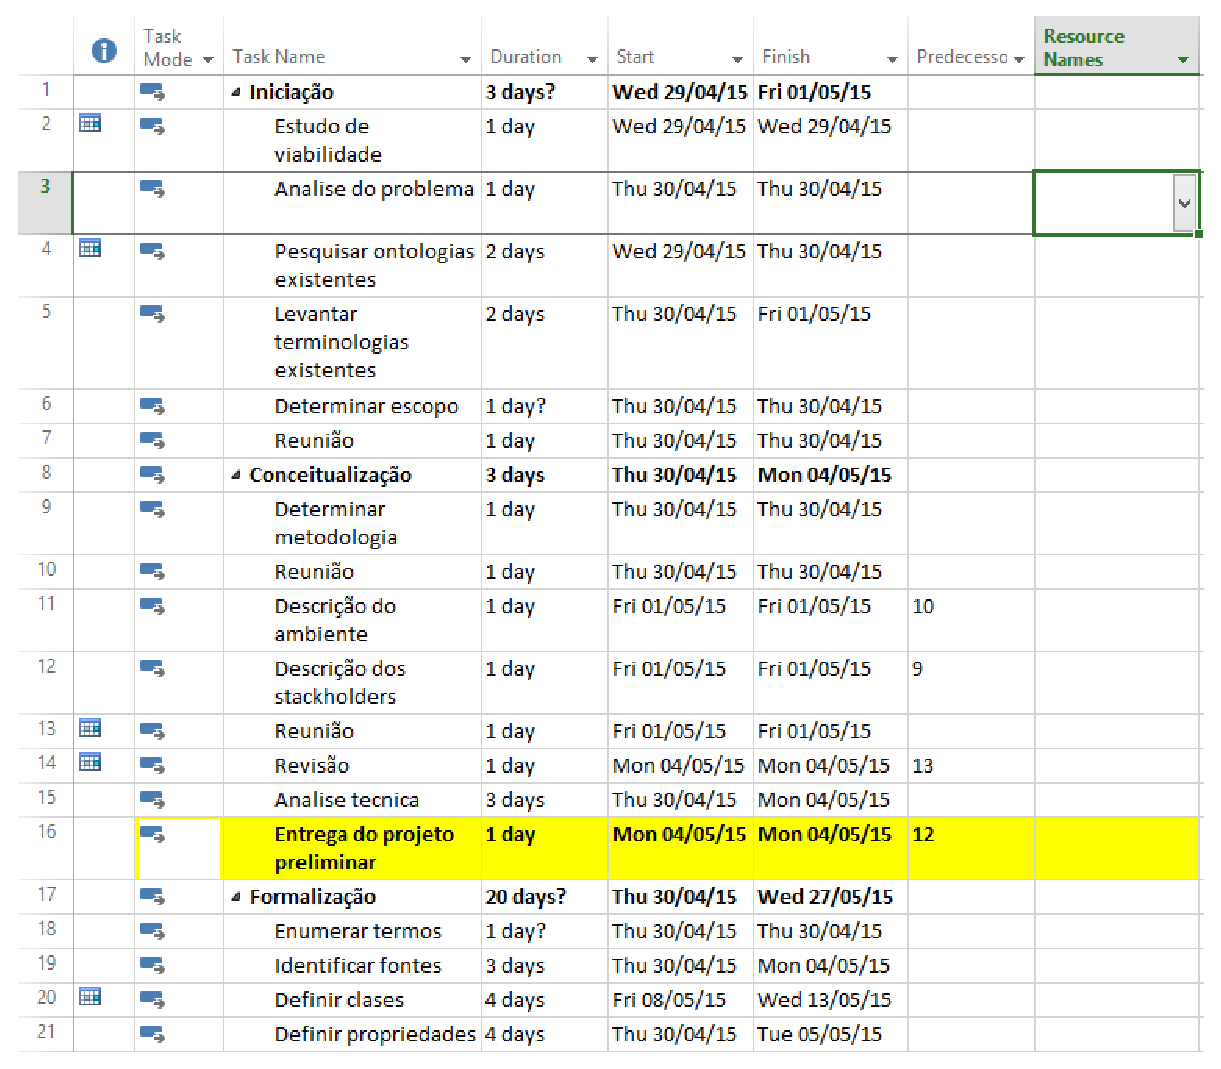
\includegraphics[keepaspectratio=true,scale=0.5]{figuras/cronograma1.eps}
  \caption{Cronograma do projeto}
\end{figure}

 \begin{figure}[ht]
  \centering
    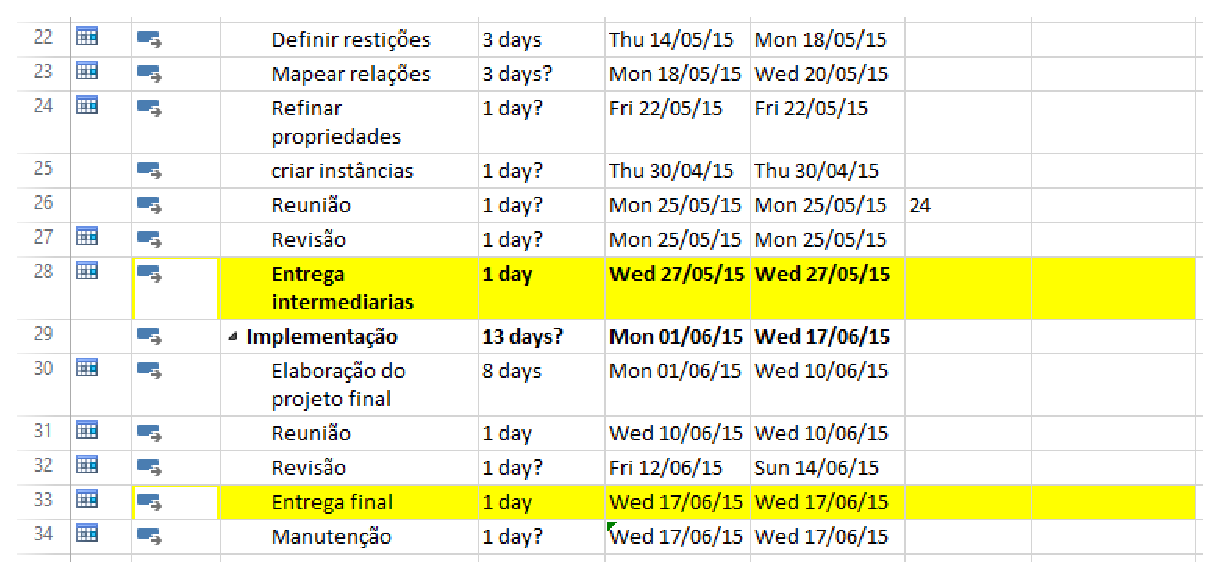
\includegraphics[keepaspectratio=true,scale=0.5]{figuras/cronograma.eps}
  \caption{Cronograma do projeto - continuação}
\end{figure}